\section{导数与微分}
\label{sec:ru-derivatives}
\label{sec:analysis-derivatives-linear-approximation}

设$f$在包含$a$的某个开区间内有定义。输入从$a$变为$a+h$时，函数增量为$\Delta f=f(a+h)-f(a)$。当$h\neq0$时，比值
\[
 \frac{\Delta f}{h}=\frac{f(a+h)-f(a)}h
\]
称为\term{差商}（difference quotient），它是这两个输入之间的平均变化率，在图像上是连接$(a,f(a))$与$(a+h,f(a+h))$的割线斜率。
让$h$趋于零，平均变化率收缩为一点处的变化率。

\begin{definition}[导数]
\label{def:ru-derivative}
若差商在$h\to0$时有有限极限，就称$f$在$a$处可导，并称
\[
 f'(a)=\lim_{h\to0}\frac{f(a+h)-f(a)}h
\]
为$f$在$a$处的\term{导数}（derivative）。若$f$在某个区间内每点可导，$x\mapsto f'(x)$称为导函数。
\end{definition}
某一点的导数是一个数，导函数是一个函数，两者不要混淆。在区间端点，或者在左右变化方式不同的点，可以只让$h>0$或只让$h<0$，分别得到右导数$f'_+(a)$与左导数$f'_-(a)$。
在内点，导数存在当且仅当左右导数都存在且相等；在闭区间的端点讨论导数时，本书总是指从区间内部取得的单侧导数。

直接计算两个例子。对$f(x)=x^2$，差商$[(a+h)^2-a^2]/h=2a+h$，令$h\to0$得$f'(a)=2a$。对$f(x)=|x|$，在原点差商为$|h|/h$：$h>0$时为$1$，$h<0$时为$-1$，
所以$f'_+(0)=1$、$f'_-(0)=-1$，绝对值函数在原点不可导，尽管它在原点连续。
反过来，可导一定连续：$f(a+h)-f(a)=\frac{f(a+h)-f(a)}h\cdot h\to f'(a)\cdot0=0$。所以连续是可导的必要条件，但不充分。
图~\ref{fig:analysis-continuity-counterexamples}比较了平方函数、绝对值函数与阶跃函数在原点的情形。
切线斜率与瞬时变化率都是导数的解释；判断导数是否存在，依据始终是差商的极限，而不是图像上看起来有没有切线。

\begin{figure*}[htbp]
 \centering
 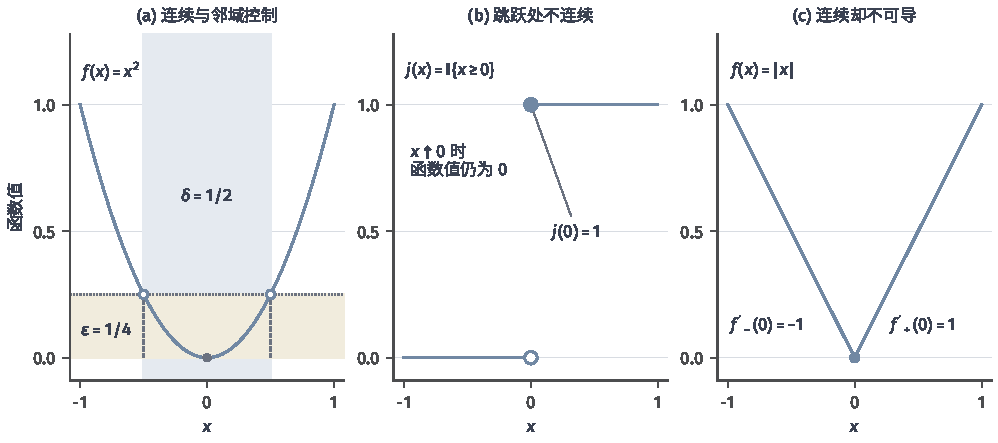
\includegraphics[width=169.0mm]{figures/01-mathematical-preliminaries-upper/02-real-numbers-and-univariate-functions/matplotlib/analysis-continuity-counterexamples/figure.pdf}
 \caption{平方函数、绝对值函数与阶跃函数在原点的差别。平方函数连续且可微；绝对值函数连续，但左右导数不同；阶跃函数的左右极限不同。连续性控制函数值的极限，可微性还要求差商具有同一个有限极限。}
 \label{fig:analysis-continuity-counterexamples}
\end{figure*}

导数的定义可以等价地改写为增量的近似形式。差商趋于$f'(a)$，等价于$[f(a+h)-f(a)-f'(a)h]/h\to0$，即
\begin{equation}
 f(a+h)=f(a)+f'(a)h+o(h),\qquad h\to0.
 \label{eq:analysis-scalar-first-order}
\end{equation}
反过来，若存在实数$A$使$f(a+h)=f(a)+Ah+o(h)$，两边减去$f(a)$、除以$h$再令$h\to0$，可知$f$可导且$A=f'(a)$。
满足这一分解的函数称为在$a$处\term{可微}（differentiable）；对一元函数，可导与可微是同一回事。
这一形式把增量分成两部分：$f'(a)h$是输入增量乘以一个固定系数，称为一次近似；余项相对于$h$可以忽略。
一元情形下，“乘以固定系数”就是最简单的线性关系；多个输入时，这个系数要换成线性映射，留到线性代数部分统一处理。

增量、微分与导数是三个不同的对象。$\Delta f$是实际的函数变化；以$f'(a)$为系数的映射$h\mapsto f'(a)h$称为$f$在$a$处的\term{微分}（differential），常记作$\mathrm df=f'(x)\,\mathrm dx$，其中$\mathrm dx$表示输入增量；
导数$f'(a)$则是这个映射的系数。
\begin{example}[平方函数在$a=3$处的微分]
\label{ex:analysis-square-differential}
设$f(x)=x^2$，$a=3$，则$f'(3)=6$，微分为$6h$。取$h=0.1$，微分给出$0.6$，实际增量为$3.1^2-3^2=0.61$，两者之差$(3+h)^2-9-6h=h^2=0.01$。
\end{example}
一次近似常用来估计误差的传递：测量半径$r$时有误差$\Delta r$，圆面积$\pi r^2$的误差约为$2\pi r\,\Delta r$。
但式~\eqref{eq:analysis-scalar-first-order}中的$o(h)$只说明$h\to0$时余项相对于$h$趋于零，并没有告诉我们在指定的$h=0.1$处余项有多大。
要得到给定步长下可以计算的误差上界，需要后面的中值定理与Taylor公式。
